% Source-authoritative solutions. N(mean,variance); Tri(min,max,mode); Exp(rate).
\makeatletter
\def\input@path{{./}{../}{../../}{../../../}{../../../../}{preamble/}{../preamble/}{../../preamble/}{../../../preamble/}{../../../../preamble/}{book2026-2027/preamble/}}
\makeatother
\input{preamble.tex}
\input{graphs/uniform_linear_probability_distributions.tex}
\input{graphs/G11_C4.tex}
\input{graphs/G11_Histograms.tex}
\usepackage{needspace}
\newgeometry{margin=0.65in,top=0.55in,bottom=0.65in}
\linespread{1.12}
\setlength{\parskip}{5pt}
\setcounter{tocdepth}{1}
\setcounter{secnumdepth}{2}
% Keep the shared scored-section interface; allow long TOC titles to wrap locally.
\renewcommand{\TOCScoredTitle}[2]{\texorpdfstring{#1\quad\sscore{#2}}{#1}}
\newcommand{\SolvedGraph}[2]{\par\smallskip\noindent\begin{minipage}{\linewidth}\centering\textbf{\small #1}\par #2\end{minipage}\par\smallskip}
% Stage numbers reset for each task; hyperlink destinations include the task name.
\newcounter{solutionstage}[section]
\renewcommand{\theHsolutionstage}{\CurrentTask.\arabic{solutionstage}}
\newcommand{\SolutionStage}[2]{\Needspace{5\baselineskip}\refstepcounter{solutionstage}%
\subsubsection*{Stage \arabic{solutionstage}: #2}\label{stage:\CurrentTask:#1}}
\newcommand{\SolutionTask}[2]{\def\CurrentTask{#1}\setcounter{solutionstage}{0}%
\Needspace{6\baselineskip}\phantomsection\label{sol:#1}\subsubsection*{Solution: #2}}
\newcommand{\TaskReturn}[1]{\par\nopagebreak[4]\begingroup\small
\noindent\hyperref[task:#1]{Return to this task}\nopagebreak[4]\secInicio[prob:\CurrentProblem]\endgroup}
% Local diagrams are needed for wraparound and the disjoint exponential tails.
\newcommand{\CycleDiagram}[4]{%
\begin{tikzpicture}[x=0.16cm,y=1cm]
\draw[->] (-1,0)--(63,0) node[right]{min};
\fill[blue!30] (0,0) rectangle (#1,0.6);
\fill[blue!30] (#2,0) rectangle (60,0.6);
\draw (0,0) rectangle (60,0.6);
\draw (0,0)--(0,-0.1) node[below]{$0$};
\draw (#1,0)--(#1,-0.1) node[below=10pt]{$#3$};
\draw (#2,0)--(#2,-0.1) node[below=10pt]{$#4$};
\draw (60,0)--(60,-0.1) node[below]{$60$};
\draw[->,thick] (59,1.0) to[bend right=12] node[above]{restart: $60\equiv0$} (1,1.0);
\end{tikzpicture}}
\newcommand{\NorthDiagram}[2]{%
\begin{tikzpicture}[scale=0.85]
\fill[blue!30] (0,0)--({90-#1}:2) arc[start angle={90-#1},end angle={90+#1},radius=2]--cycle;
\draw[thick] (0,0) circle (2);
\draw[->] (0,0)--(90:2.65) node[above]{North ($0$)};
\draw[dashed] (0,0)--({90-#1}:2.2);
\draw[dashed] (0,0)--({90+#1}:2.2);
\node[anchor=west] at ({90-#1}:2.35){$+#2$};
\node[anchor=east] at ({90+#1}:2.35){$-#2$};
\node at (0,-2.45){Full circle: $360^\circ=2\pi$ rad};
\end{tikzpicture}}
\title{Grade 11 -- Term 1\\C1--C7 Catch-up Exam Solutions\\\large Continuous distributions and sample data}
\author{Global Economics -- 2026--2027}
\date{}
\hypersetup{pdftitle={Grade 11 Term 1 C1--C7 Catch-up Exam Solutions}}
\begin{document}
\maketitle
\phantomsection\label{toc}\tableofcontents
\clearpage
\section*{Learning objective}
Identify probability distributions and their supports; use geometric interval probabilities and exponential waiting times; calculate theoretical moments, empirical probabilities, and sample statistics; and interpret errors relative to theoretical models in economic and operational contexts.\section*{Evaluated criteria}
	\textbf{C1.} Characterises discrete and continuous random variables, identifies suitable distributions and supports, and interprets density and cumulative probability in context.\par
	\textbf{C2.} Applies uniform and triangular models and constant or piecewise-linear densities to interval probabilities using geometric areas.\par
	\textbf{C3.} Uses circular geometry and arc proportions to calculate probabilities for uniform timing and directions around a circle.\par
	\textbf{C4.} Applies exponential models to constant-rate waiting times, infers event rates, and assesses model suitability.\par
	\textbf{C5.} Calculates and interprets the mean, variance, and standard deviation of continuous distributions using standard formulas.\par
	\textbf{C6.} Estimates interval probabilities using sample relative frequencies and compares them with theoretical probabilities.\par
	\textbf{C7.} Calculates sample means, variances, and standard deviations for different sample sizes and data representations and compares them with theory.
\section*{Assessment information}
Each task shows its points. Passing requires \textbf{at least 5 cumulative points per criterion, including previous learning activities}.
Show all procedures; answers without the required procedure receive no credit.
Partial credit may be awarded for a correct method with arithmetic errors.
Missing names or late submissions incur a 1-point deduction per criterion.
\begin{center}
\begin{tabular}{c|rrrrrrr|r}
Criterion&C1&C2&C3&C4&C5&C6&C7&Total\\\hline
Points&6&6&6&7&6&6&6&43
\end{tabular}
\end{center}
\textbf{Teacher note.} The source assessment table lists Problem \ref{prob:cycle} as 2 points although its heading and tasks award 3.
We follow the headings and tasks: C3 totals 6 points. The source table also lists Problem \ref{prob:receipts} as 3, but its heading and tasks award 2; C4 therefore totals 7. The source exam has not been changed.

\textbf{Conventions.} $N(\mu,\sigma^2)$ uses mean and variance;
$\operatorname{Tri}(a,b,c)$ means minimum, maximum and mode;
$\operatorname{Exp}(\lambda)$ uses the rate parameter.
Supports include their finite boundary points; endpoint inclusion does not affect continuous probabilities.
Probabilities are rounded to four decimal places (percentages to two), statistics, rates and times to three where needed, and percentage errors to two.
All errors use unrounded results. Sample variance uses $n-1$.
Blue task text links to its solution; each solution links back to its task. The arrows return to the problem and contents.

\clearpage\def\CurrentProblem{models}\sectionScored{Models in organisations}{C1-\sml{6}}{prob:models}
Colombian organisations model two random variables in each context below. \textbf{For each variable}: classify it as discrete or continuous, and identify its distribution.



\QuestionsTasks[prob:models]{
{1}/{sol:models-a}/{\phantomsection\label{task:models-a}\textbf{1. Cooperative repayments.} A cooperative records (a) whether one randomly selected member repays a monthly instalment on time, coded as 1 if timely and 0 otherwise; and (b) the number of timely repayments among 40 members. Each member repays on time independently with probability 0.92. \score{1}},
{1}/{sol:models-b}/{\phantomsection\label{task:models-b}\textbf{2. Warehouse quality checks.} A warehouse records (a) the number of invoices checked until the first incorrect invoice, including that invoice, with independent checks and a constant error probability of 0.08; and (b) a scale's measurement error between $-3$ and $3$ grams, with equal-length intervals having equal probabilities and no errors outside these limits. \score{1}},
{1}/{sol:models-c}/{\phantomsection\label{task:models-c}\textbf{3. Printing orders.} A printer records (a) the number of orders received in one hour, arriving independently at a constant rate of 2 per hour, one at a time, with multiple arrivals in a sufficiently short interval negligible; and (b) a poster order's completion time on $[10,30]$ minutes, whose density rises linearly from zero at 10 to a single peak at 18, then falls linearly to zero at 30, with no values outside this range. \score{1}},
{1}/{sol:models-d}/{\phantomsection\label{task:models-d}\textbf{4. Coffee production.} A roaster records (a) the fraction of a storage tank used at dispatch on $[0,1]$, whose density increases along one straight line from zero at 0 to its maximum at 1 and is zero elsewhere; and (b) a filling machine's measurement error, modelled by an exact symmetric bell curve on the real line, centred at 0 grams with standard deviation 4 grams. \score{1}},
{1}/{sol:models-e}/{\phantomsection\label{task:models-e}\textbf{5. Digital shop operations.} A digital shop records (a) the number of refund requests among 50 purchases, each independently resulting in a request with probability 0.04; and (b) the number of customer enquiries received over three days, arriving independently at a constant rate of 5 per day, one at a time, with multiple arrivals in a sufficiently short interval negligible. \score{1}},
{1}/{sol:models-f}/{\phantomsection\label{task:models-f}\textbf{6. Urban delivery services.} A delivery company in Bogotá studies two aspects of its daily operations. (a) Delivery times range from 15 to 45 minutes. Short deliveries are the most common, and the likelihood of observing longer delivery times decreases steadily until reaching zero at the upper limit. (b) The company also monitors the weight of its packages. Most packages weigh close to 5 kg, while lighter and heavier packages become progressively less common in a symmetric pattern. The standard deviation of package weights is 1.2 kg. \score{1}}
}

\SolutionTask{models-a}{Cooperative repayments}
\textbf{(a)} Discrete: $X\sim\operatorname{Bernoulli}(0.92)$, support $\{0,1\}$. One member gives a single timely/not-timely outcome.
\textbf{(b)} Discrete: $Y\sim\operatorname{Bin}(40,0.92)$, support $\{0,1,\ldots,40\}$. This counts successes in 40 independent trials with the same success probability.
\TaskReturn{models-a}

\SolutionTask{models-b}{Warehouse quality checks}
\textbf{(a)} Discrete: $X\sim\operatorname{Geom}(0.08)$, support $\{1,2,\ldots\}$. We count all trials up to and including the first incorrect invoice; $P(X=k)=0.92^{k-1}(0.08)$.
\textbf{(b)} Continuous: $Y\sim U(-3,3)$ grams, support $[-3,3]$ g. Equal-length intervals have equal probabilities, so $f(y)=1/6$ on the support, zero elsewhere.
\TaskReturn{models-b}

\SolutionTask{models-c}{Printing orders}
\textbf{(a)} Discrete: $X\sim\operatorname{Poisson}(2)$, support $\{0,1,2,\ldots\}$. The one-hour mean is $2\times1=2$ orders and the stated arrival conditions define a Poisson process.
\textbf{(b)} Continuous: $Y\sim\operatorname{Tri}(10,30,18)$ minutes, support $[10,30]$ min. The two straight branches and single peak specify the triangular model with mode 18.
\TaskReturn{models-c}

\SolutionTask{models-d}{Coffee production}
\textbf{(a)} Continuous: increasing-linear density on $[0,1]$, equivalently $X\sim\operatorname{Tri}(0,1,1)$. Normalisation gives $f(x)=2x$ on $[0,1]$, zero elsewhere. The fraction is unitless, and the endpoint mode is 1.
\textbf{(b)} Continuous: $Y\sim N(0,16)$ in grams, support $\mathbb R$. The exact symmetric bell curve identifies the normal model, with $\sigma=4$ g and variance $4^2=16$ g$^2$.
\TaskReturn{models-d}

\SolutionTask{models-e}{Digital shop operations}
\textbf{(a)} Discrete: $X\sim\operatorname{Bin}(50,0.04)$, support $\{0,1,\ldots,50\}$. There are 50 independent purchases with the same refund probability.
\textbf{(b)} Discrete: $Y\sim\operatorname{Poisson}(15)$, support $\{0,1,2,\ldots\}$. The three-day mean is $5\times3=15$ enquiries, rather than 5.
\TaskReturn{models-e}

\SolutionTask{models-f}{Urban delivery services}
\textbf{(a)} Continuous, support $[15,45]$ min. ``Decreases steadily'' does not uniquely establish a straight-line density. \emph{If a decreasing straight line is intended}, use $X\sim\operatorname{Tri}(15,45,15)$ with $f(x)=(45-x)/450$ on this support and zero elsewhere. Its height is $2/30=1/15$ min$^{-1}$; no extra free parameter is required under this assumption.
\textbf{(b)} Continuous package mass. Symmetric concentration around 5 kg and SD 1.2 kg do not uniquely determine a normal distribution or its full support. \emph{If a normal shape is assumed}, $Y\sim N(5,1.44)$ in kg, with model support $\mathbb R$ and variance $1.2^2=1.44$ kg$^2$. Actual package masses are nonnegative, but no exact physical support is supplied. These are intended candidates under explicit assumptions, not uniquely implied distributions.
\TaskReturn{models-f}

\clearpage\def\CurrentProblem{stall}\sectionScored{Market-stall setup}{C2-\sml{6}}{prob:stall}
The setup time $S$ for a stall at a Bogotá craft market ranges from 5 to 25 minutes. Its density is zero at both endpoints, rises linearly to its single maximum at 13 minutes, then falls linearly to zero; it is zero outside $[5,25]$.

\QuestionsTasks[prob:stall]{
{2}/{sol:stall-a}/{\phantomsection\label{task:stall-a}Find $P(9\le S\le19)$. \score{3}},
{2}/{sol:stall-b}/{\phantomsection\label{task:stall-b}Suppose the range changes to $[0,30]$, with  other properties unchanged. Recalculate $P(9\le S\le19)$. \score{3}}
}

\SolutionTask{stall-a}{Original range}
\SolutionStage{1}{Support and shape}

$S\sim\operatorname{Tri}(5,25,13)$ has support $[5,25]$ min. The density rises from $(5,0)$ to $(13,H)$ and falls to $(25,0)$.
\SolvedGraph{Support and triangular shape; horizontal coordinate in minutes}{
\CompactDensityCoordinatesGraph{3}{27}{0.13}{5,13,25}{5,13,25}{0,0.1}{s}{0,$H$}{(5,0) (13,0.1) (25,0)}}
\SolutionStage{2}{Total area = 1}
The triangle area is $\tfrac12\times\text{base}\times\text{height}$, hence
\[1=\frac12(25-5)H\quad\Longrightarrow\quad H=\frac2{20}=\frac1{10}\ \mathrm{min}^{-1}.\]
\SolutionStage{3}{Complete piecewise pdf}
For each line, use $m=(y_2-y_1)/(x_2-x_1)$ and $q=y_1-mx_1$ in $f(s)=ms+q$.
The rising branch passes through $(5,0)$ and $(13,\frac1{10})$:
\[m_1=\frac{\frac1{10}-0}{13-5}=\frac1{80},\qquad q_1=0-\frac{5}{80},\qquad f_1(s)=\frac{s-5}{80}.\]
The falling branch passes through $(13,\frac1{10})$ and $(25,0)$:
\[m_2=\frac{0-\frac1{10}}{25-13}=-\frac1{120},\qquad q_2=0-\left(-\frac1{120}\right)25=\frac{25}{120}.\]
Therefore the complete density is
\[f(s)=\begin{cases}\dfrac{s-5}{80},&5\le s\le13,\\[1mm]
\dfrac{25-s}{120},&13<s\le 25,\\[1mm]0,&\text{otherwise}.\end{cases}\]
Both branches meet at height $\frac1{10}$, are nonnegative, and have total area 1.
\Needspace{11cm}\SolutionStage{4}{Probability by complementary tail triangles}
The event straddles the mode. Remove the left triangle up to 9 and the right triangle after 19:
\[P(9\le S\le19)=1-\frac12(9-5)f(9)-\frac12(25-19)f(19).\]
Here $f(9)=4/80=1/20$ and $f(19)=6/120=1/20$ min$^{-1}$, so
\[P=1-\tfrac12(4)(1/20)-\tfrac12(6)(1/20)=1-\frac1{10}-\frac3{20}=\boxed{\frac34=0.7500=75.00\%}.\]\SolvedGraph{Shaded event: $9\le S\le19$; $s$ in minutes}{\COneGraph[s]{5}{25}{(x<=13)*((x-5)/80)+(x>13)*((25-x)/120)}{9}{19}{5,9,13,19,25}{0.13}}
Density units are inverse minutes. Integrating the two branches over $[9,13]$ and $[13,19]$ gives the same result.
\TaskReturn{stall-a}

\SolutionTask{stall-b}{Changed range}
\SolutionStage{1}{Support and shape}
\textbf{Interpretation.} ``Other properties unchanged'' retains the triangular shape and the mode at 13 minutes. Only the endpoints change to 0 and 30; the mode is not moved to 15.
$S\sim\operatorname{Tri}(0,30,13)$ has support $[0,30]$ min. The density rises from $(0,0)$ to $(13,H)$ and falls to $(30,0)$.
\SolvedGraph{Support and triangular shape; horizontal coordinate in minutes}{
\CompactDensityCoordinatesGraph{-2}{32}{0.13}{0,13,30}{0,13,30}{0,0.06666666666666667}{s}{0,$H$}{(0,0) (13,0.06666666666666667) (30,0)}}
\SolutionStage{2}{Total area = 1}
The triangle area is $\tfrac12\times\text{base}\times\text{height}$, hence
\[1=\frac12(30-0)H\quad\Longrightarrow\quad H=\frac2{30}=\frac1{15}\ \mathrm{min}^{-1}.\]
\SolutionStage{3}{Complete piecewise pdf}
For each line, use $m=(y_2-y_1)/(x_2-x_1)$ and $q=y_1-mx_1$ in $f(s)=ms+q$.
The rising branch passes through $(0,0)$ and $(13,\frac1{15})$:
\[m_1=\frac{\frac1{15}-0}{13-0}=\frac1{195},\qquad q_1=0-\frac{0}{195},\qquad f_1(s)=\frac{s-0}{195}.\]
The falling branch passes through $(13,\frac1{15})$ and $(30,0)$:
\[m_2=\frac{0-\frac1{15}}{30-13}=-\frac1{255},\qquad q_2=0-\left(-\frac1{255}\right)30=\frac{30}{255}.\]
Therefore the complete density is
\[f(s)=\begin{cases}\dfrac{s-0}{195},&0\le s\le13,\\[1mm]
\dfrac{30-s}{255},&13<s\le 30,\\[1mm]0,&\text{otherwise}.\end{cases}\]
Both branches meet at height $\frac1{15}$, are nonnegative, and have total area 1.
\Needspace{11cm}\SolutionStage{4}{Probability by complementary tail triangles}
The event straddles the mode. Remove the left triangle up to 9 and the right triangle after 19:
\[P(9\le S\le19)=1-\frac12(9-0)f(9)-\frac12(30-19)f(19).\]
Here $f(9)=9/195=3/65$ and $f(19)=11/255$ min$^{-1}$, so
\[\begin{aligned}P&=1-\tfrac12(9)(3/65)-\tfrac12(11)(11/255)\\
&=1-\frac{27}{130}-\frac{121}{510}=\boxed{\frac{368}{663}\approx0.5551=55.51\%}.\end{aligned}\]\SolvedGraph{Shaded event: $9\le S\le19$; $s$ in minutes}{\COneGraph[s]{0}{30}{(x<=13)*((x-0)/195)+(x>13)*((30-x)/255)}{9}{19}{0,9,13,19,30}{0.13}}
Density units are inverse minutes. Integrating the two branches over $[9,13]$ and $[13,19]$ gives the same result.
\TaskReturn{stall-b}

\clearpage\def\CurrentProblem{cycle}\sectionScored{A repeating inspection cycle}{C3-\sml{3}}{prob:cycle}
A cold-chain alarm occurs at a uniformly distributed position within a repeating 60-minute inspection cycle. The cycle starts at minute 0 and restarts immediately after minute 60.

\QuestionsTasks[prob:cycle]{
{3}/{sol:cycle-a}/{\phantomsection\label{task:cycle-a}Find the probability that the alarm occurs in the window from minute 52 through the restart to minute 11 of the next cycle. \score{1}},
{3}/{sol:cycle-b}/{\phantomsection\label{task:cycle-b}Find the probability that the alarm occurs within 200 seconds before or after the start of a cycle. \score{2}}
}

\SolutionTask{cycle-a}{Window through the restart}
Let $U\sim U(0,60)$ represent the position in minutes. Its density is $1/60$ min$^{-1}$ on $[0,60)$.
The restart splits the window into $[52,60)$ and $[0,11]$, with lengths $8$ and $11$ minutes.
\SolvedGraph{The shaded lengths meet through the restart}{\CycleDiagram{11}{52}{11}{52}}
\[P=\frac{(60-52)+(11-0)}{60}=\boxed{\frac{19}{60}\approx0.3167=31.67\%}.\]
\TaskReturn{cycle-a}

\SolutionTask{cycle-b}{Tolerance before and after a cycle start}
Convert units first: $200\ \mathrm{s}=200/60=10/3$ min on \emph{each} side.
The intervals are $[0,10/3]$ and $[60-10/3,60)=[170/3,60)$.
\SolvedGraph{Two equal pieces beside the cycle start}{\CycleDiagram{3.333333}{56.666667}{10/3}{170/3}}
\[P=\frac{10/3+10/3}{60}=\boxed{\frac19\approx0.1111=11.11\%}.\]
The endpoints have probability zero, so their inclusion does not change either answer.
\TaskReturn{cycle-b}

\clearpage\def\CurrentProblem{drone}\sectionScored{Direction of a survey drone}{C3-\sml{3}}{prob:drone}
A survey drone's initial heading is uniformly distributed around a full circle. A reference marker points north. ``Within an angle'' means that tolerance on \textbf{either side} of north, including wraparound.

\QuestionsTasks[prob:drone]{
{3}/{sol:drone-a}/{\phantomsection\label{task:drone-a}Compare the probability of a heading within $\pi/9$ radians of north with that of a heading within $15^\circ$ of north. Calculate both probabilities and state which exceeds the other and by how much. \score{3}}
}

\SolutionTask{drone-a}{Both angular probabilities and their comparison}
Uniform directions give probability equal to favourable angle divided by full-circle angle.
The tolerance is measured on \emph{both sides} of north.
\SolvedGraph{Two wraparound sectors centred at north}{\NorthDiagram{20}{\pi/9}\hspace{1.4cm}\NorthDiagram{15}{15^\circ}}
In radians, the event consists of $[0,\pi/9]$ and $[2\pi-\pi/9,2\pi)$:
\[P_{\pi/9}=\frac{2(\pi/9)}{2\pi}=\boxed{\frac19\approx0.1111=11.11\%}.\]
In degrees, it consists of $[0,15]$ and $[345,360)$:
\[P_{15^\circ}=\frac{2(15^\circ)}{360^\circ}=\boxed{\frac1{12}\approx0.0833=8.33\%}.\]
Thus the $\pi/9$ tolerance (20 degrees on either side) has greater probability:
\[\Delta P=\frac19-\frac1{12}=\boxed{\frac1{36}\approx0.0278},\]
an absolute difference of \textbf{2.78 percentage points}.
The relative percentage increase, using the 15-degree probability as the baseline, is
\[100\frac{1/36}{1/12}\%=33.33\%.\]
\TaskReturn{drone-a}

\clearpage\def\CurrentProblem{charging}\sectionScored{Charging-space availability}{C4-\sml{3}}{prob:charging}
Charging spaces at a logistics centre become free according to a Poisson process. The opening rate differs between the four scenarios below but remains constant within each scenario. In each case, observe from a fixed time and let $T$ be the waiting time in minutes for the next opening.

\QuestionsTasks[prob:charging]{
{4}/{sol:charging-a}/{\phantomsection\label{task:charging-a}With an average of 5 openings every 30 minutes, find the probability of waiting less than 4 minutes, $P(T<4)$. \score{0.5}},
{4}/{sol:charging-b}/{\phantomsection\label{task:charging-b}With a mean waiting time of 4 minutes between openings, find the probability of waiting more than 6 minutes, $P(T>6)$. \score{0.5}},
{4}/{sol:charging-c}/{\phantomsection\label{task:charging-c}With an average of 3 openings every 20 minutes, find the probability of waiting between 2 and 7 minutes, $P(2<T<7)$. \score{1}},
{4}/{sol:charging-d}/{\phantomsection\label{task:charging-d}With an average of 12 openings per hour, find the probability that the waiting time is outside the range from 3 to 8 minutes, $P(T<3\text{ or }T>8)$. \score{1}}
}

\Needspace{8cm}\SolutionTask{charging-a}{Less than four minutes}
The rate is $\lambda_1=5/30=1/6\approx0.167$ openings per minute.
For $T\sim\operatorname{Exp}(\lambda_1)$, $P(T<t)=1-e^{-\lambda_1t}$.
\[P(T<4)=1-e^{-(1/6)(4)}=\boxed{1-e^{-2/3}\approx0.4866=48.66\%}.\]
\SolvedGraph{Shaded left tail; $t$ in minutes and $f_T(t)$ in inverse minutes}{\ExponentialLessThanGraph{0.1666666667}{4}{6}}
\TaskReturn{charging-a}

\Needspace{8cm}\SolutionTask{charging-b}{More than six minutes}
A mean wait of 4 min gives $\lambda_2=1/E(T)=1/4=0.250$ openings per minute.
The survival formula is $P(T>t)=e^{-\lambda_2t}$.
\[P(T>6)=e^{-(1/4)(6)}=\boxed{e^{-3/2}\approx0.2231=22.31\%}.\]
\SolvedGraph{Shaded right tail; $t$ in minutes and $f_T(t)$ in inverse minutes}{\ExponentialGreaterThanGraph{0.25}{6}{6}}
The shaded tail continues beyond the plotted right edge to infinity.
\TaskReturn{charging-b}

\Needspace{8cm}\SolutionTask{charging-c}{Between two and seven minutes}
The separate rate is $\lambda_3=3/20=0.150$ openings per minute.
For an interval, $P(a<T<b)=e^{-\lambda_3 a}-e^{-\lambda_3 b}$.
\[P(2<T<7)=e^{-(3/20)(2)}-e^{-(3/20)(7)}=\boxed{e^{-3/10}-e^{-21/20}\approx0.3909=39.09\%}.\]
\SolvedGraph{Shaded middle interval; $t$ in minutes and $f_T(t)$ in inverse minutes}{\ExponentialProbabilityGraph{0.15}{2}{7}}
\TaskReturn{charging-c}

\Needspace{11cm}\SolutionTask{charging-d}{Outside three to eight minutes}
Convert the hourly rate: $\lambda_4=12/60=1/5=0.200$ openings per minute.
The tails are disjoint, so
\[P(T<a\text{ or }T>b)=(1-e^{-\lambda_4a})+e^{-\lambda_4b}.\]
\[\begin{aligned}P(T<3\text{ or }T>8)&=1-e^{-(1/5)(3)}+e^{-(1/5)(8)}\\
&=\boxed{1-e^{-3/5}+e^{-8/5}\approx0.6531=65.31\%}.\end{aligned}\]
\SolvedGraph{Both shaded tails; right tail continues to infinity}{%
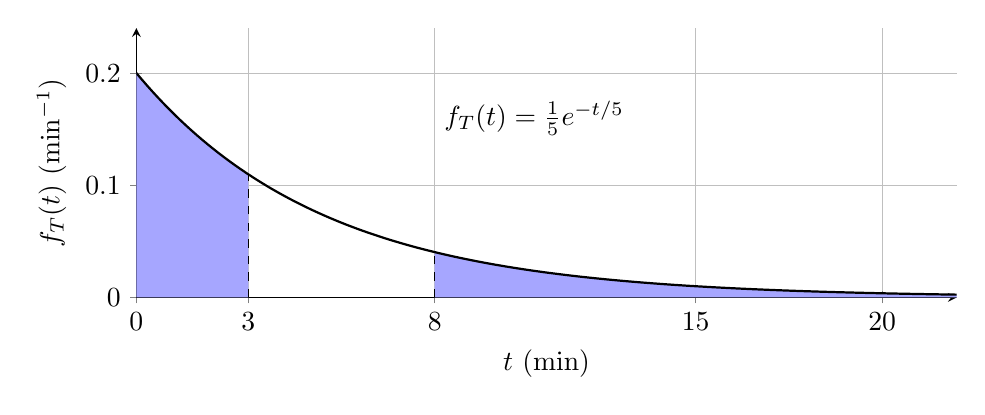
\begin{tikzpicture}\begin{axis}[width=12cm,height=5cm,axis lines=left,xmin=0,xmax=22,ymin=0,ymax=0.24,
xlabel={$t$ (min)},ylabel={$f_T(t)$ (min$^{-1}$)},xtick={0,3,8,15,20},grid=major]
\addplot[domain=0:3,samples=60,draw=none,fill=blue!35]{0.2*exp(-0.2*x)}\closedcycle;
\addplot[domain=8:22,samples=100,draw=none,fill=blue!35]{0.2*exp(-0.2*x)}\closedcycle;
\addplot[domain=0:22,samples=150,thick]{0.2*exp(-0.2*x)};
\addplot[dashed] coordinates {(3,0)(3,0.1097623)};
\addplot[dashed] coordinates {(8,0)(8,0.0403793)};
\node[anchor=west] at (axis cs:8,0.16){$f_T(t)=\frac15e^{-t/5}$};
\end{axis}\end{tikzpicture}}
For all four scenarios, $f_T(t)=\lambda e^{-\lambda t}$ for $t\ge0$ and zero otherwise; support is $[0,\infty)$.
The stated constant-rate Poisson process makes the exponential waiting-time model appropriate.
\TaskReturn{charging-d}

\Needspace{14\baselineskip}\def\CurrentProblem{receipts}\sectionScored{Electronic receipt rates}{C4-\sml{2}}{prob:receipts}
A digital shop issues electronic receipts according to a Poisson process with a constant rate during each shift. The morning and afternoon shifts have different rates. From a fixed observation time within each shift, let $T_m$ and $T_a$ be the waiting times in minutes for the next receipt in the morning and afternoon, respectively. Assume the relevant shift continues throughout each waiting time.

\QuestionsTasks[prob:receipts]{
{4}/{sol:receipts-a}/{\phantomsection\label{task:receipts-a}In the morning, $P(T_m>10)=0.40$. Infer the morning rate in receipts per hour. \score{1}},
{4}/{sol:receipts-b}/{\phantomsection\label{task:receipts-b}In the afternoon, $P(T_a<6)=0.80$. Infer the afternoon rate in receipts per hour. \score{1}}
}

\SolutionTask{receipts-a}{Morning rate from survival}
Use $P(T_m>t)=e^{-\lambda_m t}$:
\[0.40=e^{-10\lambda_m}\ \Longrightarrow\ \ln(0.40)=-10\lambda_m
\ \Longrightarrow\ \lambda_m=-\frac{\ln(0.40)}{10}\approx0.092\ \text{receipts/min}.\]
Convert minutes to hours using the exact rate:
\[60\lambda_m=-6\ln(0.40)\approx\boxed{5.498\ \text{receipts/hour}}.\]
\TaskReturn{receipts-a}

\SolutionTask{receipts-b}{Afternoon rate from a cumulative probability}
Use $P(T_a<t)=1-e^{-\lambda_a t}$:
\[0.80=1-e^{-6\lambda_a}\ \Longrightarrow\ e^{-6\lambda_a}=0.20
\ \Longrightarrow\ -6\lambda_a=\ln(0.20).\]
\[\lambda_a=-\frac{\ln(0.20)}6\approx0.268\ \text{receipts/min},\qquad
60\lambda_a=-10\ln(0.20)\approx\boxed{16.094\ \text{receipts/hour}}.\]
\TaskReturn{receipts-b}

\Needspace{14\baselineskip}\def\CurrentProblem{payments}\sectionScored{Two payment channels}{C4-\sml{2}}{prob:payments}
Completed payments on channels A and B follow independent constant-rate Poisson processes. At a fixed observation time, the probability that A's next payment occurs within 5 minutes is 0.75. The probability that B's next payment takes more than 5 minutes is 0.50. Count payments on both channels from that same observation time.

\QuestionsTasks[prob:payments]{
{4}/{sol:payments-a}/{\phantomsection\label{task:payments-a}Infer both rates. After how many minutes does A's expected payment count exceed B's expected count by 3? Find the time for this difference in expectations. \score{2}}
}

\SolutionTask{payments-a}{Rates and the difference in expected counts}
For A, the given probability is cumulative:
\[0.75=1-e^{-5\lambda_A}\ \Longrightarrow\ e^{-5\lambda_A}=0.25
\ \Longrightarrow\ \lambda_A=-\frac{\ln(0.25)}5=\frac{\ln4}{5}\approx0.277\ \text{payments/min}.\]
For B, the given probability is a survival probability:
\[0.50=e^{-5\lambda_B}\ \Longrightarrow\ \lambda_B=-\frac{\ln(0.50)}5=\frac{\ln2}{5}\approx0.139\ \text{payments/min}.\]
Define $N_A(t),N_B(t)$ as the payment counts from the common observation time.
For a constant-rate Poisson process,
\[E[N_A(t)]=\lambda_A t,\qquad E[N_B(t)]=\lambda_B t.\]
Thus $E[N_A(t)]-E[N_B(t)]=(\lambda_A-\lambda_B)t$.
\[(\lambda_A-\lambda_B)t=3\quad\Longrightarrow\quad
t=\frac{3}{\ln4/5-\ln2/5}=\boxed{\frac{15}{\ln2}\approx21.640\ \text{min}}.\]
This is the time when the \emph{difference in expectations} is 3; the actual random count difference need not equal 3 at that time.
\TaskReturn{payments-a}

\Needspace{14\baselineskip}\def\CurrentProblem{labelling}\sectionScored{Two labelling stations}{C5-\sml{2}}{prob:labelling}
At a food cooperative, let $A$ and $B$ be labelling times in minutes at two stations. Both have support $[3,15]$.

For A, the density increases along one straight line from zero at 3 to its highest value at 15. For B, equal-length time intervals within the support have equal probabilities. Both densities are zero outside $[3,15]$.

\QuestionsTasks[prob:labelling]{
{5}/{sol:labelling-a}/{\phantomsection\label{task:labelling-a}Identify A's distribution and calculate its mean, variance, and standard deviation. \score{1}},
{5}/{sol:labelling-b}/{\phantomsection\label{task:labelling-b}Identify B's distribution and calculate its mean, variance, and standard deviation. \score{1}}
}

\SolutionTask{labelling-a}{Increasing-linear labelling time}
The straight increasing density is an endpoint triangular model:
$A\sim\operatorname{Tri}(3,15,15)$, support $[3,15]$ min.
For an increasing-linear density on $[a,b]$,
\[\mu=\frac{a+2b}{3},\qquad \sigma^2=\frac{(b-a)^2}{18},\qquad\sigma=\sqrt{\sigma^2}.\]
\[E(A)=\frac{3+2(15)}3=11\ \text{min},\qquad
\operatorname{Var}(A)=\frac{(15-3)^2}{18}=8\ \text{min}^2,\qquad
\sigma_A=\sqrt8\approx2.828\ \text{min}.\]
\TaskReturn{labelling-a}

\SolutionTask{labelling-b}{Uniform labelling time}
Equal-length intervals have equal probabilities, so $B\sim U(3,15)$, support $[3,15]$ min.
The formulas are $\mu=(a+b)/2$, $\sigma^2=(b-a)^2/12$, $\sigma=\sqrt{\sigma^2}$.
\[E(B)=\frac{3+15}{2}=9\ \text{min},\qquad
\operatorname{Var}(B)=\frac{(15-3)^2}{12}=12\ \text{min}^2,\qquad
\sigma_B=\sqrt{12}\approx3.464\ \text{min}.\]
\TaskReturn{labelling-b}

\Needspace{14\baselineskip}\def\CurrentProblem{revenue}\sectionScored{Display production and daily revenue}{C5-\sml{2}}{prob:revenue}
A workshop models display production time $D$ on $[1,10]$ hours. Its density decreases along one straight line from its highest value at 1 to zero at 10 and is zero outside this support.

The workshop models daily revenue $R$, measured in \textbf{thousands of Colombian pesos (COP)}, by an exact symmetric bell curve on the real line. Its density is centred at 1800 and has inflection points at 1680 and 1920, all in thousands of COP.

\QuestionsTasks[prob:revenue]{
{5}/{sol:revenue-a}/{\phantomsection\label{task:revenue-a}Identify D's distribution and calculate its mean, variance, and standard deviation. \score{1}},
{5}/{sol:revenue-b}/{\phantomsection\label{task:revenue-b}Identify R's distribution and infer its parameters. Calculate the mean and standard deviation in \textbf{COP} and the variance in \textbf{COP$^2$}. Interpret the mean in context. \score{1}}
}

\SolutionTask{revenue-a}{Decreasing-linear production time}
The straight decreasing density is $D\sim\operatorname{Tri}(1,10,1)$, support $[1,10]$ h.
For a decreasing-linear density, $\mu=(2a+b)/3$, $\sigma^2=(b-a)^2/18$, $\sigma=\sqrt{\sigma^2}$.
\[E(D)=\frac{2(1)+10}{3}=4\ \text{h},\qquad
\operatorname{Var}(D)=\frac{(10-1)^2}{18}=\frac92=4.500\ \text{h}^2,\qquad
\sigma_D=\frac3{\sqrt2}\approx2.121\ \text{h}.\]
\TaskReturn{revenue-a}

\SolutionTask{revenue-b}{Normal revenue and conversion to COP}
The exact symmetric bell curve is normal. In thousands of COP, its centre gives $\mu_R=1800$.
A normal density's inflection points are $\mu_R\pm\sigma_R$, hence
\[\sigma_R=1920-1800=1800-1680=120,\qquad R\sim N(1800,120^2)=N(1800,14400).\]
The mathematical support is $\mathbb R$. In these units $E(R)=\mu_R$, $\operatorname{Var}(R)=\sigma_R^2$ and $\operatorname{SD}(R)=\sigma_R$.
Let $Y=1000R$ be revenue in COP. In general,
\[E(cR)=cE(R),\quad\operatorname{Var}(cR)=c^2\operatorname{Var}(R),\quad\operatorname{SD}(cR)=|c|\operatorname{SD}(R).\]
Therefore
\[E(Y)=1000(1800)=1{,}800{,}000\ \text{COP},\]
\[\operatorname{Var}(Y)=1000^2(14400)=14{,}400{,}000{,}000\ \text{COP}^2,\qquad
\operatorname{SD}(Y)=1000(120)=120{,}000\ \text{COP}.\]
The workshop's long-run average daily revenue is 1,800,000 COP; individual days vary around that average.
\TaskReturn{revenue-b}

\Needspace{14\baselineskip}\def\CurrentProblem{repairs}\sectionScored{Requests and repair times}{C5-\sml{2}}{prob:repairs}
A repair cooperative receives requests according to a constant-rate Poisson process averaging 12 requests per hour. Let $T$ be the interarrival time in minutes.

The duration $S$ of a repair has support $[10,30]$ minutes. Its density rises linearly from zero at 10 to a single peak at 18, then falls linearly to zero at 30; it is zero outside this range.

\QuestionsTasks[prob:repairs]{
{5}/{sol:repairs-a}/{\phantomsection\label{task:repairs-a}Identify T's distribution and calculate its mean and standard deviation in minutes and its variance in minutes$^2$. \score{1}},
{5}/{sol:repairs-b}/{\phantomsection\label{task:repairs-b}Identify S's distribution and calculate its mean and standard deviation in minutes and its variance in minutes$^2$. \score{1}}
}

\SolutionTask{repairs-a}{Exponential interarrival time}
The constant-rate Poisson process gives $T\sim\operatorname{Exp}(\lambda)$, support $[0,\infty)$ min,
with $\lambda=12/60=1/5=0.200$ requests/min.
The formulas are $\mu=1/\lambda$, $\sigma^2=1/\lambda^2$ and $\sigma=1/\lambda$.
\[E(T)=\frac1{1/5}=5\ \text{min},\qquad
\operatorname{Var}(T)=\frac1{(1/5)^2}=25\ \text{min}^2,\qquad
\sigma_T=\frac1{1/5}=5\ \text{min}.\]
\TaskReturn{repairs-a}

\SolutionTask{repairs-b}{Triangular repair duration}
The two straight branches give $S\sim\operatorname{Tri}(10,30,18)$, support $[10,30]$ min.
For minimum $a$, maximum $b$ and mode $c$,
\[\mu=\frac{a+b+c}{3},\qquad
\sigma^2=\frac{a^2+b^2+c^2-ab-ac-bc}{18},\qquad\sigma=\sqrt{\sigma^2}.\]
\[E(S)=\frac{10+30+18}{3}=\frac{58}{3}\approx19.333\ \text{min}.\]
\[\begin{aligned}\operatorname{Var}(S)
&=\frac{10^2+30^2+18^2-10(30)-10(18)-30(18)}{18}\\
&=\frac{304}{18}=\frac{152}{9}\approx16.889\ \text{min}^2,\end{aligned}\]
\[\sigma_S=\sqrt{152/9}=\frac{2\sqrt{38}}3\approx4.110\ \text{min}.\]
\TaskReturn{repairs-b}

\Needspace{14\baselineskip}\def\CurrentProblem{parcels}\sectionScored{Parcel masses}{C6-\sml{2}}{prob:parcels}
A sample of 50 parcel masses $X$, in kilograms, is recorded in two non-overlapping parts. The first 20 masses are listed individually:
\[
\begin{array}{rrrrr}
1.2&1.5&2.0&2.2&2.4\\
2.5&2.7&3.0&3.1&3.4\\
1.8&2.0&2.3&2.6&2.9\\
3.0&3.2&3.5&3.8&4.0
\end{array}
\]
The remaining 30 masses are summarised in a frequency table:
\[
\begin{array}{c|rrrrrr}
x_i&2.0&2.4&2.6&2.8&3.0&3.2\\\hline
f_i&3&5&7&6&5&4
\end{array}
\]

 

The model gives $P(2\le X<3)=0.40$; include 2 and exclude 3. Combine both parts as one sample.

\QuestionsTasks[prob:parcels]{
{6}/{sol:parcels-a}/{\phantomsection\label{task:parcels-a}Find the empirical probability of this event. \score{1}},
{6}/{sol:parcels-b}/{\phantomsection\label{task:parcels-b}Calculate its absolute and percentage errors. \score{1}}
}

\SolutionTask{parcels-a}{Empirical probability}
In the first part, the eligible masses are
$2.0,2.2,2.4,2.5,2.7,2.0,2.3,2.6,2.9$.
There are \textbf{9} eligible raw observations. In the table, values $2.0,2.4,2.6,2.8$ contribute $3+5+7+6=21$.
Include 2 and exclude every occurrence of 3. The parts do not overlap, so $n=20+30=50$ and $k=9+21=30$.
\[\widehat P(2\le X<3)=\frac kn=\frac{30}{50}=\frac{3}{5}=0.6000=60.00\%.\]
\TaskReturn{parcels-a}

\SolutionTask{parcels-b}{Absolute and percentage errors}
Use $E=|\widehat P-P_0|$ and $E\%=100E/|P_0|$ with the exact relative frequency.
\[E=\left|\frac{3}{5}-0.40\right|=\frac{1}{5}=0.2000.\]
\[E\%=\frac{\frac{1}{5}}{0.40}\times100\%\approx50.00\%.\]
Probabilities and their errors are unitless.
\TaskReturn{parcels-b}

\Needspace{14\baselineskip}\def\CurrentProblem{transfers}\sectionScored{File transfers, grouped data}{C6-\sml{2}}{prob:transfers}
Transfer times $X$ in seconds are grouped below. Classes include the left endpoint and exclude the right endpoint.
\[
\begin{array}{c|rrrr}
\text{Class}&[0,4)&[4,8)&[8,12)&[12,16)\\\hline
f_i&3&9&5&3
\end{array}
\]
The model gives $P(4\le X<12)=0.75$.

\QuestionsTasks[prob:transfers]{
{6}/{sol:transfers-a}/{\phantomsection\label{task:transfers-a}Find the empirical probability of this event. \score{1}},
{6}/{sol:transfers-b}/{\phantomsection\label{task:transfers-b}Calculate its absolute and percentage errors. \score{1}}
}

\SolutionTask{transfers-a}{Empirical probability}
The complete included classes are $[4,8)$ and $[8,12)$.
Thus $n=3+9+5+3=20$ and $k=9+5=14$. These are exact event counts; no midpoint approximation is needed.
\[\widehat P(4\le X<12)=\frac kn=\frac{14}{20}=\frac{7}{10}=0.7000=70.00\%.\]
\TaskReturn{transfers-a}

\SolutionTask{transfers-b}{Absolute and percentage errors}
Use $E=|\widehat P-P_0|$ and $E\%=100E/|P_0|$ with the exact relative frequency.
\[E=\left|\frac{7}{10}-0.75\right|=\frac{1}{20}=0.0500.\]
\[E\%=\frac{\frac{1}{20}}{0.75}\times100\%\approx6.67\%.\]
Probabilities and their errors are unitless.
\TaskReturn{transfers-b}

\Needspace{14\baselineskip}\def\CurrentProblem{queues}\sectionScored{Collection queues, histogram}{C6-\sml{2}}{prob:queues}
The histogram is the only supplied sample record of collection waiting times $X$ in minutes. Equal-width classes include the left endpoint and exclude the right endpoint. Bar heights are frequencies; the horizontal axis gives minutes.
\HistogramGraph{(0,2),(2,4),(4,6),(6,8)}{4,10,8,2}
{0.94\linewidth}{4.4cm}{blue!25}{2}{2}
The model gives $P(2\le X<6)=0.70$.

\QuestionsTasks[prob:queues]{
{6}/{sol:queues-a}/{\phantomsection\label{task:queues-a}Find the empirical probability of this event. \score{1}},
{6}/{sol:queues-b}/{\phantomsection\label{task:queues-b}Calculate its absolute and percentage errors. \score{1}}
}

\SolutionTask{queues-a}{Empirical probability}
Read histogram heights as frequencies: $4,10,8,2$.
The two complete included classes are $[2,4)$ and $[4,6)$.
Thus $n=4+10+8+2=24$ and $k=10+8=18$. No midpoint approximation is needed.
\[\widehat P(2\le X<6)=\frac kn=\frac{18}{24}=\frac{3}{4}=0.7500=75.00\%.\]
\TaskReturn{queues-a}

\SolutionTask{queues-b}{Absolute and percentage errors}
Use $E=|\widehat P-P_0|$ and $E\%=100E/|P_0|$ with the exact relative frequency.
\[E=\left|\frac{3}{4}-0.70\right|=\frac{1}{20}=0.0500.\]
\[E\%=\frac{\frac{1}{20}}{0.70}\times100\%\approx7.14\%.\]
Probabilities and their errors are unitless.
\TaskReturn{queues-b}

\Needspace{14\baselineskip}\def\CurrentProblem{cold-room}\sectionScored{Cold-room readings, mixed data}{C7-\sml{2}}{prob:cold-room}
A sample of 12 cold-room readings, in degrees Celsius, is recorded in two non-overlapping parts. The first five readings are $6,8,9,11,12$. The remaining seven readings are summarised below:
\[
\begin{array}{c|rrr}x_i&6&9&12\\\hline f_i&2&3&2\end{array}
\]
Combine both parts as one sample. The theoretical mean is $9\,{}^\circ\mathrm C$ and variance is $5\,({}^\circ\mathrm C)^2$.

\QuestionsTasks[prob:cold-room]{
{7}/{sol:cold-room-a}/{\phantomsection\label{task:cold-room-a}Calculate mean, variance and standard deviation. \score{1}},
{7}/{sol:cold-room-b}/{\phantomsection\label{task:cold-room-b}Calculate absolute and percentage errors for mean and variance. \score{1}}
}

\SolutionTask{cold-room-a}{Sample statistics from combined data}
The first five readings contribute one each at $6,8,9,11,12$; the frequency table adds $2,3,2$ at $6,9,12$. The combined sample has the following actual values and frequencies, so no midpoint estimation is used.\[\begin{array}{c|rrrrr}x_i&6&8&9&11&12\\\hline f_i&3&1&4&1&3\end{array}\]
Use the sample-variance denominator $n-1$, not $n$:
\[n=\sum f_i=12,\qquad\bar x=\frac{\sum f_ix_i}{n}=\frac{3(6)+1(8)+4(9)+1(11)+3(12)}{12}=\frac{109}{12}\approx9.083\ {}^\circ\mathrm C.\]
The weighted squared-deviation sum is
\[\begin{aligned}Q&=\sum_i f_i(x_i-\bar x)^2\\&=3\left(6-\frac{109}{12}\right)^2+1\left(8-\frac{109}{12}\right)^2+4\left(9-\frac{109}{12}\right)^2+1\left(11-\frac{109}{12}\right)^2+3\left(12-\frac{109}{12}\right)^2\\&=\frac{707}{12}\ ({}^\circ\mathrm C)^2.\end{aligned}\]
\begin{samepage}\[s^2=\frac{\sum_i f_i(x_i-\bar x)^2}{n-1}=\frac{\frac{707}{12}}{12-1}=\frac{707}{132}\approx5.356\ ({}^\circ\mathrm C)^2,\]
\[s=\sqrt{s^2}=\sqrt{\frac{707}{132}}\approx2.314\ {}^\circ\mathrm C.\]\end{samepage}

\TaskReturn{cold-room-a}

\SolutionTask{cold-room-b}{Mean and variance errors}
For a statistic $z$ and theoretical value $z_0$, use $E=|z-z_0|$ and $E\%=100E/|z_0|$.
Using unrounded statistics:
\[E_{\bar x}=\left|\frac{109}{12}-9\right|=\frac{1}{12}\approx0.083\ {}^\circ\mathrm C,\qquad
E_{\bar x}\%=100\frac{\frac{1}{12}}{9}\%\approx0.93\%.\]
\[E_{s^2}=\left|\frac{707}{132}-5\right|=\frac{47}{132}\approx0.356\ ({}^\circ\mathrm C)^2,\qquad
E_{s^2}\%=100\frac{\frac{47}{132}}{5}\%\approx7.12\%.\]
The requested errors concern the mean and variance only.
\TaskReturn{cold-room-b}

\Needspace{14\baselineskip}\def\CurrentProblem{routes}\sectionScored{Courier routes, grouped data}{C7-\sml{2}}{prob:routes}
Route times in minutes are grouped below. Classes include the left endpoint and exclude the right endpoint. The theoretical mean is 14 minutes and variance is 12 minutes$^2$.
\[
\begin{array}{c|rrr}
\text{Class}&[8,12)&[12,16)&[16,20)\\\hline
f_i&2&3&1
\end{array}
\]

\QuestionsTasks[prob:routes]{
{7}/{sol:routes-a}/{\phantomsection\label{task:routes-a}Calculate mean, variance and standard deviation. \score{1}},
{7}/{sol:routes-b}/{\phantomsection\label{task:routes-b}Calculate absolute and percentage errors for mean and variance. \score{1}}
}

\SolutionTask{routes-a}{Sample statistics from class midpoints}
The class midpoint is $(\text{left}+\text{right})/2$. Individual observations are unavailable, so all three statistics and their errors below are \textbf{midpoint estimates}.\[\begin{array}{c|rrr}m_i&10&14&18\\\hline f_i&2&3&1\end{array}\]
Use the sample-variance denominator $n-1$, not $n$:
\[n=\sum f_i=6,\qquad\bar x=\frac{\sum f_im_i}{n}\approx\frac{2(10)+3(14)+1(18)}{6}=\frac{40}{3}\approx13.333\ \mathrm{min}.\]
The weighted squared-deviation sum is
\[\begin{aligned}Q&=\sum_i f_i(m_i-\bar x)^2\\&=2\left(10-\frac{40}{3}\right)^2+3\left(14-\frac{40}{3}\right)^2+1\left(18-\frac{40}{3}\right)^2\\&=\frac{136}{3}\ \mathrm{min}^2.\end{aligned}\]
\begin{samepage}\[s^2=\frac{\sum_i f_i(m_i-\bar x)^2}{n-1}\approx\frac{\frac{136}{3}}{6-1}=\frac{136}{15}\approx9.067\ \mathrm{min}^2,\]
\[s=\sqrt{s^2}\approx\sqrt{\frac{136}{15}}\approx3.011\ \mathrm{min}.\]\end{samepage}

\TaskReturn{routes-a}

\SolutionTask{routes-b}{Mean and variance errors}
For a statistic $z$ and theoretical value $z_0$, use $E=|z-z_0|$ and $E\%=100E/|z_0|$.
Using unrounded midpoint estimates:
\[E_{\bar x}=\left|\frac{40}{3}-14\right|=\frac{2}{3}\approx0.667\ \mathrm{min},\qquad
E_{\bar x}\%=100\frac{\frac{2}{3}}{14}\%\approx4.76\%.\]
\[E_{s^2}=\left|\frac{136}{15}-12\right|=\frac{44}{15}\approx2.933\ \mathrm{min}^2,\qquad
E_{s^2}\%=100\frac{\frac{44}{15}}{12}\%\approx24.44\%.\]
The requested errors concern the mean and variance only.
\TaskReturn{routes-b}

\Needspace{14\baselineskip}\def\CurrentProblem{containers}\sectionScored{Reusable-container masses}{C7-\sml{2}}{prob:containers}
The histogram is the only supplied sample record of container masses in kilograms. Equal-width classes include the left endpoint and exclude the right endpoint. Bar heights are frequencies; the horizontal axis gives kilograms. The theoretical mean is 7 kg and variance is 4 kg$^2$.
\HistogramGraph{(4,6),(6,8),(8,10),(10,12)}{2,3,2,1}
{0.94\linewidth}{4.4cm}{orange!30}{2}{1}

\QuestionsTasks[prob:containers]{
{7}/{sol:containers-a}/{\phantomsection\label{task:containers-a}Calculate mean, variance and standard deviation. \score{1}},
{7}/{sol:containers-b}/{\phantomsection\label{task:containers-b}Calculate absolute and percentage errors for mean and variance. \score{1}}
}

\SolutionTask{containers-a}{Sample statistics from class midpoints}
The class midpoint is $(\text{left}+\text{right})/2$. Individual observations are unavailable, so all three statistics and their errors below are \textbf{midpoint estimates}.\[\begin{array}{c|rrrr}m_i&5&7&9&11\\\hline f_i&2&3&2&1\end{array}\]
Use the sample-variance denominator $n-1$, not $n$:
\[n=\sum f_i=8,\qquad\bar x=\frac{\sum f_im_i}{n}\approx\frac{2(5)+3(7)+2(9)+1(11)}{8}=\frac{15}{2}\approx7.500\ \mathrm{kg}.\]
The weighted squared-deviation sum is
\[\begin{aligned}Q&=\sum_i f_i(m_i-\bar x)^2\\&=2\left(5-\frac{15}{2}\right)^2+3\left(7-\frac{15}{2}\right)^2+2\left(9-\frac{15}{2}\right)^2+1\left(11-\frac{15}{2}\right)^2\\&=30\ \mathrm{kg}^2.\end{aligned}\]
\begin{samepage}\[s^2=\frac{\sum_i f_i(m_i-\bar x)^2}{n-1}\approx\frac{30}{8-1}=\frac{30}{7}\approx4.286\ \mathrm{kg}^2,\]
\[s=\sqrt{s^2}\approx\sqrt{\frac{30}{7}}\approx2.070\ \mathrm{kg}.\]\end{samepage}

\TaskReturn{containers-a}

\SolutionTask{containers-b}{Mean and variance errors}
For a statistic $z$ and theoretical value $z_0$, use $E=|z-z_0|$ and $E\%=100E/|z_0|$.
Using unrounded midpoint estimates:
\[E_{\bar x}=\left|\frac{15}{2}-7\right|=\frac{1}{2}\approx0.500\ \mathrm{kg},\qquad
E_{\bar x}\%=100\frac{\frac{1}{2}}{7}\%\approx7.14\%.\]
\[E_{s^2}=\left|\frac{30}{7}-4\right|=\frac{2}{7}\approx0.286\ \mathrm{kg}^2,\qquad
E_{s^2}\%=100\frac{\frac{2}{7}}{4}\%\approx7.14\%.\]
The requested errors concern the mean and variance only.
\TaskReturn{containers-b}


\clearpage\section{Summarized Solutions}\label{sec:summary}
Exact parameters and counts are retained. See the linked problems for procedures and supports.
\subsection*{C1 -- All twelve variables}
Problem \ref{prob:models}. D = discrete; C = continuous.
\begin{center}\begin{tabular}{ccll}
\toprule Context&Variable&Class&Model (parameters as defined above)\\\midrule
1&a&D&Bernoulli$(0.92)$\\
1&b&D&Binomial$(40,0.92)$\\
2&a&D&Geometric$(0.08)$, trials including the first incorrect invoice\\
2&b&C&$U(-3,3)$ g\\
3&a&D&Poisson$(2)$ orders per hour\\
3&b&C&$\operatorname{Tri}(10,30,18)$ min\\
4&a&C&Increasing-linear: $f(x)=2x$ on $[0,1]$\\
4&b&C&$N(0,16)$, in grams\\
5&a&D&Binomial$(50,0.04)$\\
5&b&D&Poisson$(15)$ enquiries over three days\\
6&a&C&Candidate $\operatorname{Tri}(15,45,15)$ min if linearity is assumed\\
6&b&C&Candidate $N(5,1.44)$, in kg, if normality is assumed\\\bottomrule
\end{tabular}\end{center}
Context 6 is not uniquely determined: monotone decrease need not be linear, and symmetry with SD 1.2 kg need not be normal. The normal candidate has support $\mathbb R$; physical mass is nonnegative and its precise support is not supplied.

\subsection*{C2 -- Triangular models}
Problem \ref{prob:stall}. Both models have mode 13 min and are zero outside their respective supports.
\[
\begin{array}{c|c|c|c}
\text{Support/model}&\text{Rising pdf}&\text{Falling pdf}&P(9\le S\le19)\\\hline
[5,25],\ \operatorname{Tri}(5,25,13)&(s-5)/80&(25-s)/120&3/4=0.7500=75.00\%\\
{}[0,30],\ \operatorname{Tri}(0,30,13)&s/195&(30-s)/255&368/663\approx0.5551=55.51\%
\end{array}
\]
Rising branches end at 13; falling branches start after 13. Heights are $1/10$ and $1/15$ min$^{-1}$.

\clearpage\subsection*{C3 -- Cycles and directions}
Problem \ref{prob:cycle}: restart window $[52,60)\cup[0,11]$ has probability $19/60\approx0.3167=31.67\%$.
The 200-second tolerance on each side gives $[0,10/3]\cup[170/3,60)$ and probability $1/9\approx0.1111=11.11\%$.

Problem \ref{prob:drone}: $P_{\pi/9}=1/9\approx0.1111=11.11\%$;
$P_{15^\circ}=1/12\approx0.0833=8.33\%$.
The former exceeds the latter by $1/36\approx0.0278$, or 2.78 percentage points (relative increase 33.33\%).

\subsection*{C4 -- Waiting probabilities and inferred rates}
Problem \ref{prob:charging}. Rates below are openings/minute.
\begin{center}\begin{tabular}{ccll}
\toprule Scenario&Rate&Exact probability&Decimal and percentage\\\midrule
1&$1/6$&$P(T<4)=1-e^{-2/3}$&0.4866; 48.66\%\\
2&$1/4$&$P(T>6)=e^{-3/2}$&0.2231; 22.31\%\\
3&$3/20$&$P(2<T<7)=e^{-3/10}-e^{-21/20}$&0.3909; 39.09\%\\
4&$1/5$&$P(T<3\text{ or }T>8)=1-e^{-3/5}+e^{-8/5}$&0.6531; 65.31\%\\\bottomrule
\end{tabular}\end{center}
Problem \ref{prob:receipts}: morning $\lambda_m=-\ln(0.40)/10\approx0.092$ receipts/min, $60\lambda_m\approx5.498$ receipts/hour.
Afternoon $\lambda_a=-\ln(0.20)/6\approx0.268$ receipts/min, $60\lambda_a\approx16.094$ receipts/hour.

Problem \ref{prob:payments}: $\lambda_A=\ln4/5\approx0.277$ and $\lambda_B=\ln2/5\approx0.139$ payments/min.
The expected-count difference is 3 at $t=15/\ln2\approx21.640$ min.

\clearpage\subsection*{C5 -- Theoretical moments}
Supports: $A,B\in[3,15]$ min; $D\in[1,10]$ h; revenue's normal support $\mathbb R$;
$T\in[0,\infty)$ min; repair $S\in[10,30]$ min.
\begin{center}\begin{tabular}{clrrrl}
\toprule Problem&Variable/model&Mean&Variance&SD&Units\\\midrule
\ref{prob:labelling}&$A\sim\operatorname{Tri}(3,15,15)$&11&8&2.828&min; min$^2$\\
\ref{prob:labelling}&$B\sim U(3,15)$&9&12&3.464&min; min$^2$\\
\ref{prob:revenue}&$D\sim\operatorname{Tri}(1,10,1)$&4&4.500&2.121&h; h$^2$\\
\ref{prob:repairs}&$T\sim\operatorname{Exp}(1/5)$&5&25&5&min; min$^2$\\
\ref{prob:repairs}&$S\sim\operatorname{Tri}(10,30,18)$&19.333&16.889&4.110&min; min$^2$\\\bottomrule
\end{tabular}\end{center}
Units are first for mean and SD, second for variance. Exact repair moments: $58/3$, $152/9$ and $2\sqrt{38}/3$.
Problem \ref{prob:revenue}, revenue: $R\sim N(1800,14400)$ in thousands of COP, with SD 120.
In COP: mean $1{,}800{,}000$, variance $14{,}400{,}000{,}000$ COP$^2$, SD $120{,}000$ COP.
The mean is the long-run average daily revenue.

\subsection*{C6 -- Empirical probabilities}
$E=|\widehat P-P_0|$, $E\%=100E/|P_0|$. Counts use complete event classes, not midpoints.
\begin{center}\begin{tabular}{clrrrrrr}
\toprule Problem&Event&$n$&$k$&$\widehat P$&$P_0$&$E$&$E\%$\\\midrule
\ref{prob:parcels}&$2\le X<3$ kg&50&30&0.6000&0.4000&0.2000&50.00\%\\
\ref{prob:transfers}&$4\le X<12$ s&20&14&0.7000&0.7500&0.0500&6.67\%\\
\ref{prob:queues}&$2\le X<6$ min&24&18&0.7500&0.7000&0.0500&7.14\%\\\bottomrule
\end{tabular}\end{center}
Parcel counts: 9 eligible raw masses plus 21 table observations, including 2 and excluding 3.

\clearpage\subsection*{C7 -- Sample statistics and requested errors}
All sample variances use $n-1$. Asterisks mark midpoint estimates because individual observations are unavailable.
\begin{center}\begin{tabular}{crrrrl}
\toprule Problem&$n$&$\bar x$&$s^2$&$s$&Units\\\midrule
\ref{prob:cold-room}&12&9.083&5.356&2.314&$^\circ$C; $(^\circ\mathrm C)^2$\\
\ref{prob:routes}$^*$&6&13.333&9.067&3.011&min; min$^2$\\
\ref{prob:containers}$^*$&8&7.500&4.286&2.070&kg; kg$^2$\\\bottomrule
\end{tabular}\end{center}
Exact statistics $(\bar x,s^2)$: $(109/12,707/132)$, $(40/3,136/15)$, $(15/2,30/7)$.
\begin{center}\begin{tabular}{clrrl}
\toprule Problem&Statistic&Absolute error&Percentage error&Absolute-error units\\\midrule
\ref{prob:cold-room}&Mean&0.083&0.93\%&$^\circ$C\\
&Variance&0.356&7.12\%&$(^\circ\mathrm C)^2$\\
\ref{prob:routes}$^*$&Mean&0.667&4.76\%&min\\
&Variance&2.933&24.44\%&min$^2$\\
\ref{prob:containers}$^*$&Mean&0.500&7.14\%&kg\\
&Variance&0.286&7.14\%&kg$^2$\\\bottomrule
\end{tabular}\end{center}
\secInicio[sec:summary]
\end{document}
